% ============================================================================
% COURS 02 — MODÉLISATION DES MÉCANISMES
% Recomposition fidèle du document Word 2-ModelisationMecanismes2022.docx.
% Les schémas de liaisons normalisées utilisent Style/cinematique.sty.
% ============================================================================

\pagelayout{wide}
\setcounter{chapter}{2}
\setcounter{section}{0}

\definecolor{TLCycleBlue}{RGB}{78,139,199}
\definecolor{TLSectionBlue}{RGB}{35,146,166}
\definecolor{TLSubsectionOrange}{RGB}{203,118,0}
\definecolor{TLDefinitionPurple}{RGB}{115,55,155}
\definecolor{TLSoftOrange}{RGB}{252,238,224}
\definecolor{TLSoftBlue}{RGB}{235,244,250}
\definecolor{TLTableHeader}{RGB}{202,218,238}

\newcommand{\TLCheck}{\(\bigcirc\)}
\newcommand{\TLImage}[2][0.88\linewidth]{%
  \begin{center}
    \includegraphics[width=#1,height=.34\textheight,keepaspectratio]{#2}
  \end{center}
}
\newcommand{\TLImageSmall}[2][0.58\linewidth]{%
  \begin{center}
    \includegraphics[width=#1,height=.25\textheight,keepaspectratio]{#2}
  \end{center}
}
\newcommand{\TLSectionLabel}[1]{\label{TL-course-section-#1}}

\newtcolorbox{TLDefinition}[1][Définition]{
  enhanced,breakable,
  colback=TLDefinitionPurple!5,
  colframe=TLDefinitionPurple,
  boxrule=.9pt,arc=3mm,
  title={#1},
  colbacktitle=TLDefinitionPurple!8,
  coltitle=TLDefinitionPurple,
  fonttitle=\bfseries,
  attach boxed title to top center={yshift=-2mm},
  boxed title style={arc=2mm,boxrule=.9pt},
  left=4mm,right=4mm,top=4mm,bottom=3mm
}
\newtcolorbox{TLRemark}[1][Remarque]{
  enhanced,breakable,
  colback=TLSoftBlue,
  colframe=TLCoverBlue,
  boxrule=.7pt,arc=2mm,
  title={#1},fonttitle=\bfseries,
  colbacktitle=TLCoverBlue,coltitle=white,
  left=4mm,right=4mm,top=3mm,bottom=3mm
}
\newtcolorbox{TLQuoteBox}{
  enhanced,breakable,
  colback=TLSoftOrange,
  colframe=TLSubsectionOrange!65!black,
  boxrule=.6pt,arc=2mm,
  left=8mm,right=8mm,top=5mm,bottom=5mm,
  fontupper=\large\centering
}

% Symboles normalisés issus de cinematique.sty.
\newcommand{\TLSymPivot}{%
  \begin{tikzpicture}[baseline=-.5ex,scale=.65]\scPivotx{L}{(0,0)}\end{tikzpicture}}
\newcommand{\TLSymPivotGlissant}{%
  \begin{tikzpicture}[baseline=-.5ex,scale=.65]\scPivotGlissantx{L}{(0,0)}\end{tikzpicture}}
\newcommand{\TLSymGlissiere}{%
  \begin{tikzpicture}[baseline=-.5ex,scale=.65]\scGlissierex{L}{(0,0)}\end{tikzpicture}}
\newcommand{\TLSymHelicoidale}{%
  \begin{tikzpicture}[baseline=-.5ex,scale=.65]\scHelicoidalex{L}{(0,0)}\end{tikzpicture}}
\newcommand{\TLSymAppuiPlan}{%
  \begin{tikzpicture}[baseline=-.5ex,scale=.70]\scAppuiPlan{L}{(0,0)}\end{tikzpicture}}
\newcommand{\TLSymSpherePlan}{%
  \begin{tikzpicture}[baseline=-.5ex,scale=.70]\scSpherePlan{L}{(0,0)}\end{tikzpicture}}
\newcommand{\TLSymCylindrePlan}{%
  \begin{tikzpicture}[baseline=-.5ex,scale=.70]\scCylindrePlanx{L}{(0,0)}\end{tikzpicture}}
\newcommand{\TLSymSphereCylindre}{%
  \begin{tikzpicture}[baseline=-.5ex,scale=.70]\scSphereCylindrex{L}{(0,0)}\end{tikzpicture}}
\newcommand{\TLSymSpherique}{%
  \begin{tikzpicture}[baseline=-.5ex,scale=.70]\scSpherique{L}{(0,0)}\end{tikzpicture}}
\newcommand{\TLSymSpheriqueDoigt}{%
  \begin{tikzpicture}[baseline=-.5ex,scale=.70]\scSpheriqueDoigt{L}{(0,0)}\end{tikzpicture}}

\newcommand{\TLTorseur}[7]{%
  \(\left\{\mathcal V\right\}
  =\left\{\begin{array}{cc}
  #1 & #4\\
  #2 & #5\\
  #3 & #6
  \end{array}\right\}_{#7}\)
}

% Bandeau de cycle, fidèle au document Word, sur les pages de contenu.
\newcommand{\TLModelisationHeader}{%
  \ifnum\value{page}>1\relax
  \begin{tikzpicture}[remember picture,overlay]
    \fill[TLCycleBlue]
      ([xshift=82mm,yshift=-10mm]current page.north west)
      -- ([xshift=94mm,yshift=-3mm]current page.north west)
      -- ([yshift=-3mm]current page.north east)
      -- ([yshift=-17mm]current page.north east)
      -- ([xshift=82mm,yshift=-17mm]current page.north west) -- cycle;
    \node[anchor=east,text=white,font=\sffamily\bfseries\small,xshift=-9mm,yshift=-10mm]
      at (current page.north east) {Cycle 2 : Modélisation des mécanismes};
  \end{tikzpicture}%
  \fi
}
\AddToShipoutPictureFG{\TLModelisationHeader}

\section*{Objectifs du cours}
\addcontentsline{toc}{section}{Objectifs du cours}

\begin{tcolorbox}[
  enhanced,breakable,
  colback=white,colframe=TLCoverBlue,
  boxrule=.8pt,arc=2mm,
  title={Modéliser et analyser le comportement cinématique d'un mécanisme},
  colbacktitle=TLCoverBlue,coltitle=white,fonttitle=\bfseries
]
L'objectif est de savoir construire et exploiter un \textbf{schéma cinématique}
et/ou un \textbf{graphe de liaisons}.
\end{tcolorbox}

\begin{minipage}[t]{.48\linewidth}
\textbf{\large Savoirs — Je connais :}
\begin{itemize}
  \item les noms des dix liaisons usuelles ; \hfill\TLCheck
  \item leurs symboles de représentation 2D et 3D ; \hfill\TLCheck
  \item la forme générale de leurs torseurs cinématiques ; \hfill\TLCheck
  \item les symboles des transmetteurs usuels ; \hfill\TLCheck
  \item la modélisation des guidages par roulements ; \hfill\TLCheck
  \item la démarche d'élaboration d'un schéma cinématique. \hfill\TLCheck
\end{itemize}
\end{minipage}\hfill
\begin{minipage}[t]{.48\linewidth}
\textbf{\large Savoir-faire — Je sais :}
\begin{itemize}
  \item identifier et caractériser une liaison usuelle ; \hfill\TLCheck
  \item repérer les classes d'équivalence cinématique ; \hfill\TLCheck
  \item identifier la géométrie d'un contact ; \hfill\TLCheck
  \item modéliser les mouvements relatifs entre deux CEC ; \hfill\TLCheck
  \item réaliser un graphe des liaisons ; \hfill\TLCheck
  \item élaborer un schéma cinématique ; \hfill\TLCheck
  \item déterminer une liaison équivalente. \hfill\TLCheck
\end{itemize}
\end{minipage}

\section{MISE EN SITUATION}\TLSectionLabel{1}

\subsection{Cas n\textsuperscript{o}1 : lenteur d'un robot de chirurgie}

Même si elle n'est pas encore aussi répandue en France qu'aux États-Unis,
la chirurgie robotique se développe progressivement. Son usage nécessite
la maîtrise de la machine et une familiarisation avec sa manipulation,
mais également la prise en compte de contraintes telles que la durée de
l'intervention. Un arrêt de la cour administrative d'appel de Lyon du
29 septembre 2016 rappelle que l'allongement de la durée d'une opération,
lié à l'installation du robot et à un maniement hésitant, peut être en lien
direct avec les dommages subis.

\TLImage[.72\linewidth]{images/image5.jpeg}

Pour de nombreux systèmes, en particulier en robotique industrielle ou
grand public, un enjeu majeur consiste à respecter la \textbf{cinématique}
imposée par le cahier des charges : mouvements suivant des directions
déterminées, amplitudes et vitesses maîtrisées.

\TLImage[.76\linewidth]{images/image6.png}

On cherche donc à établir des relations entre les \textbf{ordres} envoyés
aux pré-actionneurs de la chaîne de puissance et la
\textbf{cinématique imposée aux effecteurs}.

\subsection{Cas n\textsuperscript{o}2 : prothèse transtibiale}

La prothèse transtibiale doit permettre à la personne de réaliser des
mouvements comparables à ceux d'un pied réel, en termes d'amplitude,
de vitesse et d'accélération.

\begin{center}
\begin{minipage}{.43\linewidth}\centering
  
\includegraphics[width=.72\linewidth,height=.24\textheight,keepaspectratio]{images/image7.jpeg}\\
  \emph{Prothèse transtibiale}
\end{minipage}\hfill
\begin{minipage}{.53\linewidth}
\begin{TLQuoteBox}
Pour maîtriser les positions et les vitesses, il faut pouvoir
\textbf{modéliser les différents mouvements du mécanisme}.
\end{TLQuoteBox}
\end{minipage}
\end{center}

\section{INTRODUCTION À LA MODÉLISATION CINÉMATIQUE}\TLSectionLabel{2}

\subsection{Définitions et hypothèses}

\begin{TLDefinition}
\textbf{Mécanisme :} ensemble des solides de la chaîne de puissance situés
entre l'actionneur et l'effecteur, assurant le transfert de puissance mécanique.
\end{TLDefinition}

\begin{TLDefinition}
\textbf{Solide ou classe d'équivalence cinématique (CEC) :} pièce ou ensemble
de pièces assemblées entre elles et ne présentant aucun mouvement relatif.
\end{TLDefinition}

Lors de l'utilisation d'un mécanisme, les solides se déforment sous l'action
des efforts. Dans ce cours, ces déformations sont supposées suffisamment
faibles pour être négligées : les solides sont considérés
\textbf{indéformables}.

\begin{TLDefinition}
Un solide indéformable \(S\) vérifie :
\[
\forall t,\ \forall A,B\in S,\qquad AB=\text{constante}.
\]
\end{TLDefinition}

\begin{TLRemark}
Cette hypothèse ne convient pas aux pièces dont la fonction est précisément
de se déformer : ressorts, barres de torsion, rondelles élastiques, etc.
\end{TLRemark}

\subsection{Modèle cinématique}

L'étude du comportement cinématique d'un mécanisme s'appuie sur un modèle,
généralement constitué d'un \textbf{schéma cinématique} et/ou d'un
\textbf{graphe des liaisons}.

\TLImage[.78\linewidth]{images/image12.png}

Ces représentations simplifiées sont utilisées aussi bien pour analyser un
système existant que pour concevoir un nouveau système. Elles constituent
des outils efficaces de communication scientifique.

\subsection{Schéma cinématique d'un mécanisme}

Un schéma cinématique propose une représentation géométrique du modèle.
Il précise les mouvements possibles entre les solides, les liaisons et les
positions relatives de ces liaisons dans l'espace.

\begin{itemize}
  \item les liaisons sont représentées par des symboles normalisés ;
  \item les solides sont représentés par des traits reliant ces symboles.
\end{itemize}

\begin{center}
\begin{minipage}[t]{.46\linewidth}\centering
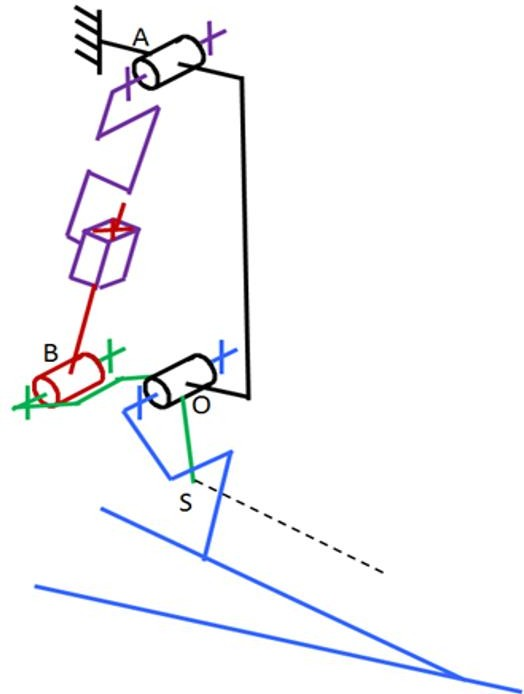
\includegraphics[width=\linewidth,height=.28\textheight,keepaspectratio]{images/image14.jpeg}\\
\emph{Schéma cinématique 3D}
\end{minipage}\hfill
\begin{minipage}[t]{.46\linewidth}\centering
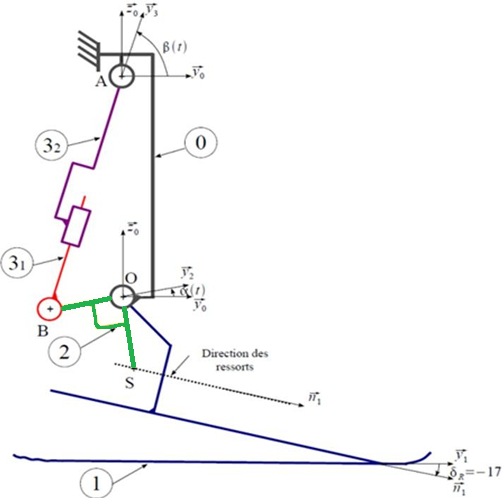
\includegraphics[width=\linewidth,height=.28\textheight,keepaspectratio]{images/image13.png}\\
\emph{Schéma cinématique 2D}
\end{minipage}
\end{center}

Le schéma peut être plan ou spatial. Il comporte également les points,
vecteurs et droites nécessaires au paramétrage.

\subsection{Graphe de liaisons d'un mécanisme}

Un graphe des liaisons représente les CEC par des nœuds et les liaisons par
des arêtes portant leurs caractéristiques géométriques.

\begin{TLQuoteBox}
Une liaison entre deux solides possède toujours exactement deux couleurs.
\end{TLQuoteBox}

\begin{center}
\begin{minipage}[t]{.56\linewidth}\centering
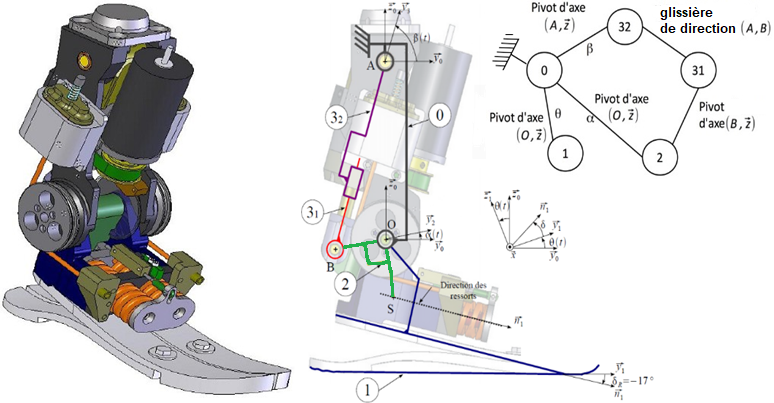
\includegraphics[width=\linewidth,height=.27\textheight,keepaspectratio]{images/image12.png}
\end{minipage}\hfill
\begin{minipage}[t]{.38\linewidth}
\begin{itemize}
  \item les solides sont les \textbf{nœuds} ;
  \item les liaisons sont les \textbf{arêtes} ;
  \item le bâti est le solide de référence.
\end{itemize}
\end{minipage}
\end{center}

Le graphe est plus simple à tracer car il ne représente pas la géométrie.
Il contient néanmoins la même information cinématique que le schéma associé.

\subsubsection*{Chaînes de solides ouvertes, fermées et complexes}

\begin{tabularx}{\linewidth}{|>{\centering\arraybackslash}X|>{\centering\arraybackslash}X|>{\centering\arraybackslash}X|}
\hline
\rowcolor{TLTableHeader}
\textbf{Chaîne ouverte} & \textbf{Chaîne fermée} & \textbf{Chaîne complexe}\\ \hline
Les solides extrêmes sont différents. &
Le solide initial est aussi le solide final. &
Plusieurs chaînes ouvertes ou fermées sont associées.\\

\includegraphics[width=.32\linewidth]{images/image15.png} &

\includegraphics[width=.32\linewidth]{images/image15.png} &

\includegraphics[width=.32\linewidth]{images/image15.png}\\
Exemple : robot & Exemple : antenne radar & Exemple : simulateur de vol\\ \hline
\end{tabularx}
